\newSec[MusterFassade]{Fassade}{3}

Die Klasse \CodeClass{PoseController} kann als Fassade angesehen werden, da hier die Interaktion mit den darin verwalteten Klassen gekapselt wird.

\missing[fällt evtl raus??]





\newSec{Klassifikation}{4}




\newSec{Struktur und beteiligte Akteure}{4}

\begin{figure}[ht!]
\vspace{0.25cm}
\begin{center}
\fbox{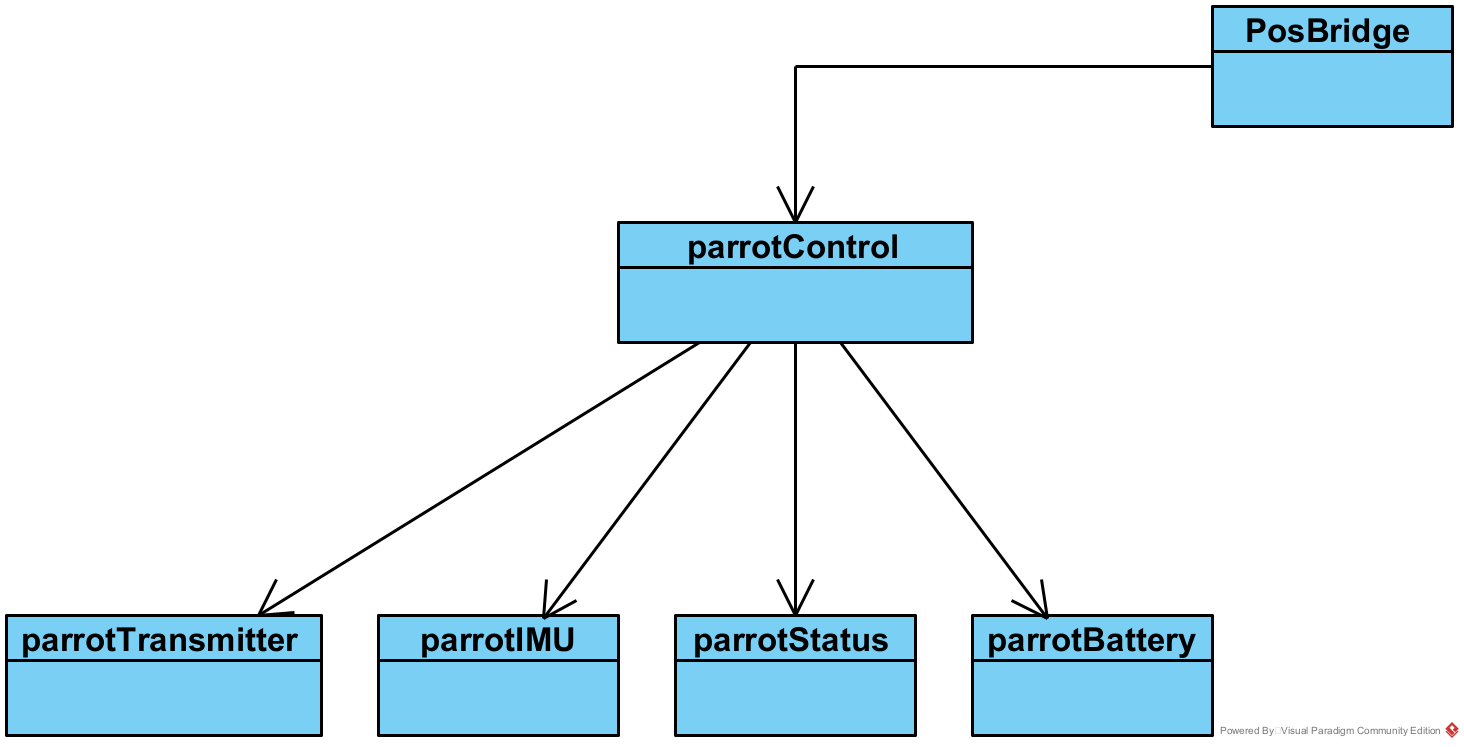
\includegraphics[width=15cm]{Pictures/Fassade.png}}
\caption{Fassade im Projekt}
\label{fig:Fas}
\end{center}

\vspace{0.25cm}
\refImgShort{fig:Fas} zeigt \missing\
\end{figure}



\newSec{Motivation}{4}

Auch hier Design-Entscheidung. Interaktion mit einer Klasse ist einfacher, als sich um alles selbst kümmern zu müssen.




